\section{Introduction} 
% \begin{itemize}
%     \item In contextual bandits the goal is to take an action A based on some contextual information X to then maximize the outcome Y.
%     \item This setup is common in many real-world settings such as healthcare, personalized recommendation systems, and online advertising, etc \citep{li2010contextual, bastani2019online, xu2020contextual}, where the goal is to take actions i.e. taking a drug or recommending an item which subsequently leads to a desirable outcome such as the patients health or click in recommendations.
%     \item However a question arises when we want to change and update the policy. Hence, in the recent years much of research has been spent on evaluating how a new policy will do based on the collected data up to now. In particular, this is also known as the field of off-policy evaluation.
% \end{itemize}
% \begin{wrapfigure}{r}{0.5\textwidth}
%     \centering
%     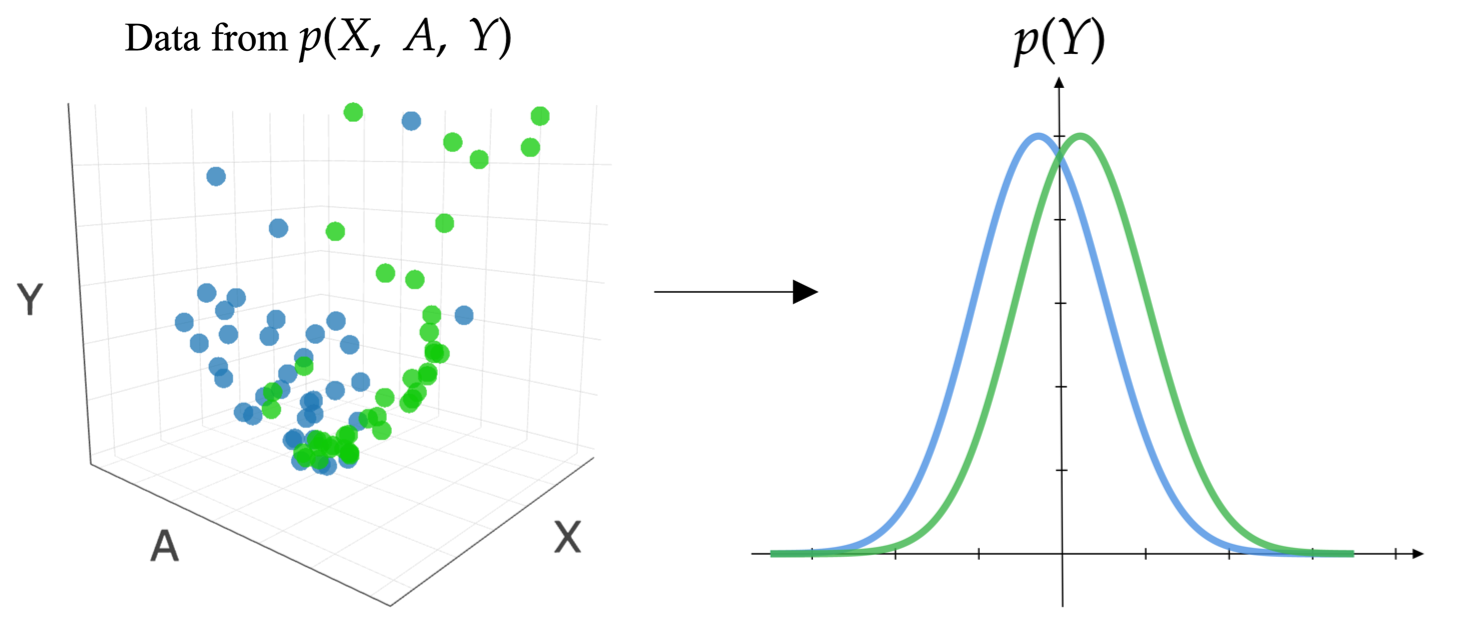
\includegraphics[width=0.5\textwidth]{figures/mr/main_pic.png}
%     \caption{Caption}
%     % \vspace{-1cm}
%     \label{fig:my_label}
% \end{wrapfigure}
In contextual bandits, the objective is to select an action $A$, guided by contextual information $X$, to maximize the resulting outcome $Y$. This paradigm is prevalent in many real-world applications such as healthcare, personalized recommendation systems, or online advertising \citep{li2010contextual, bastani2019online, xu2020contextual}. The objective is to perform actions, such as prescribing medication or recommending items, which lead to desired outcomes like improved patient health or higher click-through rates. Nonetheless, updating the policy presents challenges, as na\"ively implementing a new, untested policy may raise ethical or financial concerns. For instance, prescribing a drug based on a new policy poses risks, as it may result in unexpected side effects. As a result, recent research \citep{swaminathan2015counterfactual, wang2017optimal, farajtabar2018more, su2019continuous, metelli2021subgaussian, liu2019triply, sugiyama2012machine, swaminathan2017off} has concentrated on evaluating the performance of new policies (target policy) using only existing data that was generated using the current policy (behaviour policy). This problem is known as Off-Policy Evaluation (OPE).


Current OPE methods in contextual bandits, such as the Inverse Probability Weighting (IPW) \citep{horvitz1952generalization} and Doubly Robust (DR) \citep{dudik2014doubly} estimators primarily account for the policy shift by re-weighting the data using the ratio of the target and behaviour polices to estimate the target policy value. This can be problematic as it may lead to high variance in the estimators in cases of substantial policy shifts. The issue is further exacerbated in situations with large action or context spaces \citep{saito2022off}, since in these cases the estimation of policy ratios is even more difficult leading to extreme bias and variance.
% The problem is worsened in the policy ratios are even harder to estimate in these cases. 
% even when the distribution of outcome $Y$ changes minimally.
% \jef{Nonetheless, these methods possess a fundamental limitation, as they explicitly account for the shift between behavior and target policies when estimating the expected target policy value.} 
% As a result, the estimators may demonstrate high variance in cases of substantial policy shifts, even when the outcome distribution in $Y$ changes minimally. 
% This high variance in estimators can lead to unreliable and potentially vacuous outputs. 

% In light of these concerns, since our goal is to estimate the expected outcome $Y$ under a new target policy, we show that directly considering the shift in the marginal distribution of outcomes $Y$ rather than the shift in the policies leads to a more efficient estimator.

% Given our goal of estimating the expected outcome $Y$ under a new target policy, we show that directly considering the shift in the marginal distribution of outcomes $Y$

In this work we show that this problem of high variance in OPE can be alleviated by using methods which directly consider the shift in the marginal distribution of the outcome $Y$ resulting from the policy shift, instead of considering the policy shift itself (as in IPW and DR). To this end, we propose a new OPE estimator for contextual bandits called the Marginal Ratio (MR) estimator, which weights the data directly based on the shift in the marginal distribution of outcomes $Y$ and consequently is much more robust to increasing sizes of action and context spaces than existing methods like IPW or DR. 
% Since our goal is to estimate the expected outcome $Y$ under a new target policy, we show that 
% the problem of high variance that arises as a result of weighting the data using policy ratios can be circumvented by instead weighting the data directly based on the shift in the marginal distribution of outcomes $Y$.
% the problem of high variance can be alleviated by weighting the data directly based on the shift in the marginal distribution of outcomes $Y$ resulting from the policy shift rather than the policy ratios (as in IPW or DR).
% directly considering the shift in the marginal distribution of outcomes $Y$ rather than 
% To this end, we propose a new OPE estimator for contextual bandits called the Marginal Ratio (MR) estimator, which directly takes into account the shift in the marginal distribution of the outcome and consequently is much more robust to increasing sizes of action and context spaces than existing methods like IPW or DR. 
Our extensive theoretical analyses show that MR enjoys better variance properties than the existing methods making it highly attractive for a variety of applications in addition to OPE. One such application is the estimation of Average Treatment Effect (ATE) in causal inference, for which we show that MR provides greater sample efficiency than the most commonly used methods.

Our contributions in this paper are as follows:
% and can also be used in domains like causal inference for the estimation of Average Treatment Effect (ATE) where it leads to desirable properties such as increased sample efficiency 
% Additionally, we theoretically show that MR enjoys better variance properties than
% achieves significant variance reduction compared to 
% conventional methods (like IPW or DR) and consequently is much more robust to increasing sizes of action and context spaces.
% Additionally, we also show that the MR estimator can be applied in causal inference for the estimation of Average Treatment Effect (ATE). We demonstrate theoretically and empirically that the MR estimator is more sample efficient than existing methods. Our contributions in this paper are:



% by weighting the samples based on how relevant the observed \emph{outcome} is to the target outcome distribution.

% Our proposed method aims to offer a more robust solution, mitigating the adverse effects of high variance and providing a reliable alternative to existing OPE techniques. 
% At a high level, instead of weighting the samples based on the policy shift as in IPW, the MR estimator weights the samples based on how relevant the observed \emph{outcome} is to target outcome distribution.

% Current OPE methods in contextual bandits, such as the inverse propensity weighting (IPW) \citep{horvitz1952generalization} and doubly robust (DR) \citep{dudik2014doubly} estimators, have gained considerable popularity in practice due to their ability to estimate the expected value of a modified policy. However, these methods have an inherent limitation, as they explicitly consider the shift between behavior and target policies when estimating the target policy value. Consequently, the estimators can exhibit high variance when there is a significant policy shift, even if the change in the outcome distribution is minimal. This issue can be especially pronounced in scenarios with large action or context spaces \citep{saito2022off}.



% Contextual bandits are a prevalent framework \jef{need to rewrite this banditS are A framework doesnt sound right} used in several real-world applications, including healthcare, personalized recommendation systems, and online advertising \citep{li2010contextual, bastani2019online, xu2020contextual}\faaiz{more refs}. In this setup, an agent takes actions $A$ based on contextual information $X$, and receives outcomes $Y$ accordingly. In such settings \jef{Two times start with IN}, evaluating the effectiveness of a new policy without actually deploying it is often desirable \jef{Due to potential financial or ethical reasons + refs}. \jef{Would start this with: Hence, in recent years, researchers have ... }Off-policy evaluation (OPE) is a popular approach that estimates the expected value of a \jef{a or the?} random variable $Y$ under a target policy $\tar$, without deploying the target policy \citep{swaminathan2015counterfactual, wang2017optimal, farajtabar2018more, su2019continuous, metelli2021subgaussian, liu2019triply, sugiyama2012machine, swaminathan2017off}.

% Current OPE methods in contextual bandits focus on the shift in the joint distribution of the context, action, and outcome when estimating the expected value \jef{this sentence is coming out of nowhere}. These methods, such as the inverse propensity weighting (IPW) \citep{horvitz1952generalization} and doubly robust (DR) \citep{dudik2014doubly} estimators, have been highly popular in practice \jef{This should come first}. However, they have a fundamental limitation: they explicitly take the shift between behaviour and target policies into account when estimating target policy value. \jef{we might want to be more vague here in case people do not understand the problem of the ratios, or we have to be way more concrete}


% \jef{I will use AB review from now on :) }


% do not only take the shift in the distribution of the outcome into account, but also the shift in the distribution of the actions. 
% As a result, the estimators can have high variance when the policy shift is large, even if the shift in the outcome distribution is small. This issue can be particularly pronounced in large action or context spaces \citep{saito2022off}.

% To address this limitation, we propose a new OPE estimator for contextual bandits that only takes into account the shift in the marginal distribution of the outcome as a result of the policy shift. Our estimator, called Marginal Ratio (MR) estimator, utilizes the available logged data more efficiently and leads to lower variance than the current state-of-the-art methods. At a high level, instead of weighting the samples based on the policy shift as in IPW, the MR estimator weights the samples based on how relevant the observed \emph{outcome} is to target outcome distribution.
% assigns high weights to the samples where the observed outcomes are most relevant to the target outcome distribution.  

\begin{itemize}
    \item Firstly, we introduce MR, an OPE estimator for contextual bandits, that focuses on the shift in the marginal distribution of $Y$ rather than the joint distribution of $(X, A, Y)$. 
    \flag{We show that MR has favourable theoretical properties compared to existing methods like IPW and DR. Our analysis also encompasses theory on the approximation errors of our estimator. 
    % that MR achieves lower variance than conventional OPE methods like IPW.
    }
    % We provide extensive theoretical comparisons to show  the variance reduction properties of MR compared to existing approaches such as IPW and DR.
    % at MR achieves lower variance than IPW and DR estimators. 
    
    \item Secondly, we explicitly lay out the connection between MR and  Marginalized Inverse Propensity Score (MIPS) \cite{saito2022off}, a recent state-of-the-art contextual bandits OPE method, and prove that MR attains lowest variance among a generalized family of MIPS estimators. 
    \item Thirdly, we show that the MR estimator can be applied in the setting of causal inference to estimate average treatment effects (ATE), and theoretically prove that the resulting estimator is more data-efficient with higher accuracy and lower variance than commonly used methods. 
    \item Finally, we verify all our theoretical analyses through a variety of experiments on synthetic and real-world datasets and empirically demonstrate that the MR estimator achieves better overall performance compared to current state-of-the-art methods. 
\end{itemize}
% Firstly, we introduce MR, an OPE estimator for contextual bandits that focuses on the shift in the marginal distribution of $Y$ rather than the joint distribution of $(X, A, Y)$. Specifically, we provide extensive theoretical comparisons which show that MR achieves lower variance than classical importance-weighted estimators like IPW and DR. Our analysis also encompasses theory on the estimation errors of our estimator. Secondly, we explicitly layout the connection between MR and  Marginalized Inverse Propensity Score (MIPS) \cite{saito2022off}, a recent state-of-the-art contextual bandits OPE method, and demonstrate that MR attains lowest variance among a generalized family of MIPS estimators. Thirdly, we show that the MR estimator can be applied in the setting of causal inference to estimate average treatment effects (ATE), and theoretically prove that the resulting estimator is more data-efficient with higher accuracy and lower variance than commonly used methods. Finally, we verify all our theoretical analyses through a variety of experiments on synthetic and real-world datasets and empirically demonstrate that the MR estimator achieves better overall performance compared to current state-of-the-art methods. 

%  Our contributions in this paper are fourfold.
% \begin{enumerate}[label=\roman*.]
%     \item We introduce MR, an OPE estimator for contextual bandits that focuses on the shift in the marginal distribution of $Y$ rather than the joint distribution of $(X, A, Y)$. Specifically, we provide extensive theoretical comparisons 
%     which show that MR achieves lower variance than classical importance-weighted estimators like IPW and DR.
%     Our analysis also encompasses theory on the estimation errors of our estimator.
%     % In addition, we provide convergence rates for our estimator.
%     % Moreover, we show that MR is likely to achieve lower variance than the DR method when the dimensions of context $X$ are large.
%     % \item We provide theoretical results comparing the performance of MR against the most commonly used OPE estimators for contextual bandits. We prove that the variance of our estimator is lower than that of the classical importance-weighted estimator (IPW). Additionally, we contrast MR against the recently proposed MIPS estimator \citep{saito2022off} and show that MR achieves the optimal variance over the class of all MIPS estimators.
%     \item We explicitly layout the connection between MR and  Marginalized Inverse Propensity Score (MIPS) \cite{saito2022off}, a current state-of-the-art contextual bandits OPE method, and demonstrate that MR attains lowest variance among a generalized family of MIPS estimators.
%     \item We show that the MR estimator can be applied in the setting of causal inference to estimate average treatment effects (ATE), and theoretically prove that the resulting estimator is more data-efficient with higher accuracy and lower variance than commonly used methods.
%     \item We verify all our theoretical analyses through a variety of experiments on synthetic and real-world datasets and empirically demonstrate that the MR estimator achieves better overall performance compared to current state-of-the-art methods.
%     % \item We show that the MR estimator can be applied in the setting of causal inference to estimate average treatment effects (ATE), and leads to a more data-efficient estimator with higher accuracy and lower variance than the most commonly used methods.
%     % \item We verify our analysis on a variety of experiments on synthetic datasets as well as real-world datasets. We empirically show that MR achieves better performance overall compared to the current state-of-the-art methods.
% \end{enumerate}

% First, we propose a new off-policy evaluation (OPE) estimator, called MR, which only takes into account the shift in the marginal distribution of $Y$ instead of the joint distribution of $(X, A, Y)$. Second, we provide theoretical results comparing the performance of MR against the most commonly used OPE estimators for contextual bandits. We prove that the variance of our estimator is lower than that of the classical importance-weighted estimator (IPW). Additionally, we contrast MR against the recently proposed MIPS estimator \citep{saito2022off} and show that MR achieves the optimal variance over the class of all MIPS estimators. Third, we show that the MR estimator can be applied in the setting of causal inference to estimate average treatment effects (ATE), and leads to a more data-efficient estimator with high accuracy and low variance than the most commonly used methods.  Finally, we verify our analysis on a variety of experiments on synthetic datasets as well as real-world datasets. We empirically show that MR achieves better performance overall compared to the current state-of-the-art methods. 
% Our proposed method, MR, can therefore be seen as a significant contribution to the field of off-policy evaluation for contextual bandits.

% Specifically, we provide theoretical results showing that the variance of MR is lower than those of the classical IPW estimator, and the recently proposed MIPS estimator \citep{saito2022off}. We also show that MR achieves the optimal variance over the class of all MIPS estimators.

% In addition to the theoretical analysis, we evaluate the performance of MR on both synthetic and real-world classification datasets. Our experiments demonstrate that MR achieves better performance overall compared to the existing methods. Overall, our proposed MR estimator presents a significant contribution to the OPE problem in contextual bandits, providing a more efficient and accurate way to estimate the expected value of a random variable under a target policy
